\begin{center}
\fbox{\fbox{\parbox{6.5in}{\centering
\begin{flushleft}

\vspace{2mm}
\hspace{5mm}
\textbf{\underline{Kahe sirge lõikamine kolmandaga}}

\vspace{2mm}
\hspace{5mm}
Kui meil on kaks sirget $s$ ja $t$ lõigatud kolmanda sirgega $u$, mida nimetame \textbf{lõikajaks}, siis tekib meil\\ \hspace{5mm} kaheksa nurka.

\begin{center}
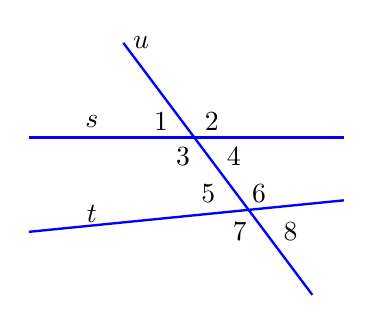
\begin{tikzpicture}[scale=0.4]

\draw[line width=0.3mm, blue] (0,0) to (10,0);
\node[above] at (2,0) {$s$};

\draw[line width=0.3mm, blue] (0,-3) to (10,-2);
\node[above] at (2, -3){$t$};

\draw[line width=0.3mm, blue] (3,3) to (9,-5);
\node[right] at (3,3){$u$};

\node at (5,0.5){$1$ \quad $2$};
\node at (5.7,-0.6){$3$ \quad $4$};
\node at (6.5,-1.8){$5$ \quad $6$};
\node at (7.5,-3){$7$ \quad $8$};
\end{tikzpicture}
\end{center}

\hspace{5mm}
Teame, et tippunurgad on võrdsed. Järelikult: $\angle 1=\angle 4$, $\angle 2 = \angle 3$, $\angle 5 = \angle 8$ ja $ \angle 6 = \angle 7$.

\hspace{5mm}
Asendame võrdsed nurgad nurkadega $\alpha$, $\beta$, $\gamma$, $\delta$.


\begin{center}
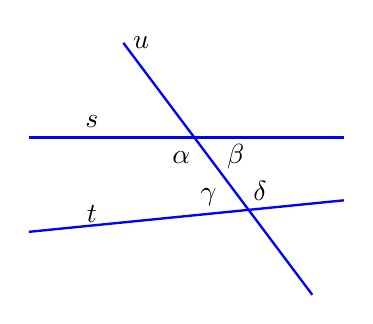
\begin{tikzpicture}[scale=0.4]

\draw[line width=0.3mm, blue] (0,0) to (10,0);
\node[above] at (2,0) {$s$};

\draw[line width=0.3mm, blue] (0,-3) to (10,-2);
\node[above] at (2, -3){$t$};

\draw[line width=0.3mm, blue] (3,3) to (9,-5);
\node[right] at (3,3){$u$};

\node at (5.7,-0.6){$\alpha$ \quad $\beta$};
\node at (6.5,-1.8){$\gamma$ \quad $\delta$};
\end{tikzpicture}
\end{center}

\hspace{5mm}
Nurki, mille haarad lõikajal on vastassuunalised ja mis asuvad ühel pool lõikajat, nimetatakse\\ \hspace{5mm} \textbf{lähisnurkadeks}. Meie joonisel on lähisnurkadeks nurgad $\alpha$ ja $\delta$ ning $\beta$ ja $\gamma$.

\vspace{2mm}
\hspace{5mm}
Nurki, mille haarad lõikajal on vastassuunalised ja mis asuvad teine teisel pool lõikajat, nimetatakse\\ \hspace{5mm} \textbf{põiknurkadeks}. Meie joonisel on põiknurkadeks nurgad $\alpha$ ja $\gamma$ ning $\beta$ ja $\delta$.

\vspace{5mm}
\hspace{5mm}
\textbf{\underline{Teoreemid}}

\vspace{2mm}
\hspace{5mm}
1) Kui üks paar põiknurki on võrdsed, siis on võrdsed ka teine paar põiknurki.


\begin{center}
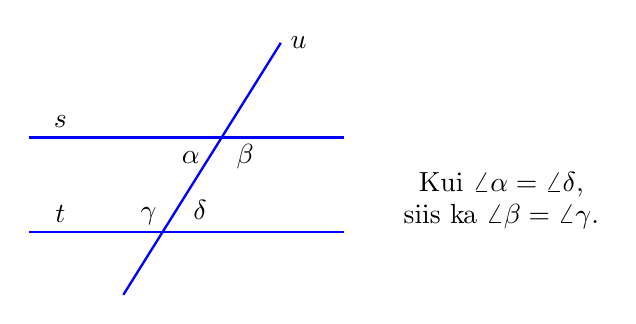
\begin{tikzpicture}[scale=0.4]

\draw[line width=0.3mm, blue] (0,0) to (10,0);
\node[above] at (1,0) {$s$};

\draw[line width=0.3mm, blue] (0,-3) to (10,-3);
\node[above] at (1, -3){$t$};

\draw[line width=0.3mm, blue] (8,3) to (3,-5);
\node[right] at (8,3){$u$};

\node at (6,-0.6){$\alpha$ \quad $\beta$};
\node at (4.6,-2.4){$\gamma$ \quad $\delta$};

\node at (15,-1.5){Kui $\angle \alpha = \angle \delta$,};
\node at (15,-2.5){siis ka $\angle \beta = \angle \gamma$.};

\end{tikzpicture}
\end{center}



\vspace{2mm}
\hspace{5mm}
2) Kui põiknurgad on võrdsed, siis lähisnurkade summa ona  $180^{o}$.

\end{flushleft}
}}}
\end{center}

\pagebreak

\begin{center}
\fbox{\fbox{\parbox{6.5in}{\centering
\begin{flushleft}

\vspace{2mm}
\hspace{5mm}
\textbf{\underline{Sirgete paralleelsuse tunnused}}

\vspace{2mm}
\hspace{5mm}
\textbf{Sirgete paralleelsuse I tunnus}

\vspace{2mm}
\hspace{5mm}
Kaks sirget on paralleelsed siis ja ainult siis, kui nende lõikamisel kolmanda sirgega tekivad võrdsed\\ \hspace{5mm} põiknurgad.

\vspace{2mm}
\hspace{5mm}
\textbf{Sirgete paralleelsuse II tunnus}

\vspace{2mm}
\hspace{5mm}
Kaks sirget on paralleelsed siis ja ainult siis, kui nende lõikamisel kolmanda sirgega tekkinud\\ \hspace{5mm} lähisnurkade summa on $180^{o}$.



\end{flushleft}
}}}
\end{center}


\vspace{0.5cm}

\textbf{Märkmed}\\
\vspace{2mm}
\begin{mdframed}[style=graphpaper]
\vspace{15cm}
\end{mdframed}